\documentclass[11pt,letterpaper]{report}
\usepackage[pdftex]{graphicx}
\usepackage[version=3]{mhchem}
\usepackage{tabularx}
\usepackage{multirow}
\usepackage{amssymb} %this is used to get \therefore
\usepackage{capt-of}


\newcommand{\HRule}{\rule{\linewidth}{0.5mm}}
\setlength{\topmargin}{-.7in}
\setlength{\leftmargin}{-.7in}
\setlength{\textheight}{9in}
\setlength{\oddsidemargin}{0in}
\setlength{\textwidth}{6.25in}
\newcommand{\degree}{\ensuremath{^\circ}}



\begin{document}

\begin{titlepage}
\begin{center}

\textsc{\Large Experiment 5}\\[1.5cm]
\textsc{\Large Grossmont College - Chemistry 141}\\[0.5cm]

\HRule \\[0.4cm]
{ \LARGE \bfseries Analysis of a Two Component Alloy}\\[0.5cm]

\HRule \\[1.5cm]

\begin{minipage}{0.4\textwidth}
\begin{flushleft} \large
\emph{Author:}\\
Cameron \textsc{Carroll}
\end{flushleft}
\end{minipage}
\begin{minipage}{0.4\textwidth}
\begin{flushright} \large
\emph{Instructor \& Class:}\\
Judy \textsc{George} - 141 (8844)
\end{flushright}
\end{minipage}

\vfill

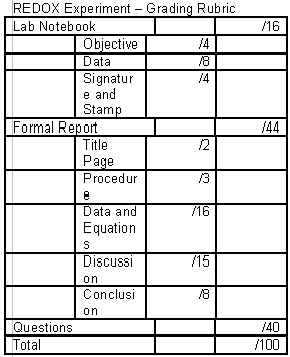
\includegraphics{./redox_rxn_rubric.png}\\[1cm]

{\large \today}

\end{center}
\end{titlepage}
\pagebreak

\section*{Objective}
This experiment is an exploration in using the ideal gas law in mass percent calculations; The hydrogen gas evolved from two metals in an alloy reacting with hydrochloric acid is used to determine the percent composition of that alloy. By taking measurements before and after the reaction, one can determine the composition of the reactant alloy.

\section*{Introduction}

Dalton's law of partial pressure states that the total pressure of a gas is equal to the sum of its parts. These partial pressures are assumed not to react with each other, and all gases are ideal. In the context of this experiment, Dalton's law is used to find the pressure of hydrogen gas evolved in the system. Hydrogen gas, evolved from the reaction between alloy and acid, is the primary source of pressure in the system. The water vapor, however, in its continuous dynamic, must also be accounted for to achieve an accurate result. 

The ideal gas law, stemming from the kinetic molecular theory, is a fundamental part of this experiment. Using the collected data and the pressure, obtained using Dalton's law, one can then calculate the moles of hydrogen evolved in total. All of the variables are measurable or constant except for the moles of hydrogen produced, which easily follows from the formula $n = \frac{PV}{RT}$

\section*{Procedure \& Safety:}

\paragraph{Procedure:}
Lehman, J; Olmstead, T; Vance, D; (2011)
Experiment 8: Analysis of a two-component alloy
Chemistry 141 Lab Manual (Edition 5.2) (Pages 8-65 - 8-70)

\paragraph{Hazardous Material and Safety Notes:}
\begin{itemize}
\item Closed-toe shoes and safety goggles are required at all times. \\[-0.5cm]
\item Experiment generates hydrogen gas, and should be performed in a fume hood. It is prone to explosion if lit. \\[-0.5cm]
\item Generator flask solution should be disposed of in inorganic hazardous waste. \\[-0.5cm]
\end{itemize}


\section*{Data:}
\begin{center}
\captionof{table}{Intermediate Data}
\label{table1}
\vspace{0.3cm}
\begin{tabularx}{\textwidth}{ | m{1cm}| X| X| X| X| X|}
\hline
\textsc{Trial} & \textsc{Sample Weight} & \textsc{Water difference} & \textsc{Temperature gas} & \textsc{Temperature water} & \textsc{Mass Water Displaced} \\
\hline
1 & 1.813 g & 0.8 cm & 21.0\degree c & 18.5\degree c & 1104 g \\
2 & 1.689 g & 0.8 cm & 21.1\degree c & 19.0\degree c & 1197 g \\
3 & 1.800 g & 5.3 cm & 21.0\degree c & 20.0\degree c & 1568 g \\
4 & 1.282 g & 2.3 cm & 19.0\degree c & 18.5\degree c & 1122 g \\
\hline
\multicolumn{5}{|l|}{Barometric Pressure:} & 740.1 mm Hg \\
\multicolumn{5}{|l|}{Density of Water:} & 0.998 g/mL \\
\hline
\end{tabularx}
\end{center}

\vspace{1cm}

\begin{center}
\captionof{table}{Calculated Results}
\label{table2}
\vspace{0.3cm}
\begin{tabularx}{\textwidth}{ | m{1cm}| X| X| X|}
\hline
\textsc{Trial} & \textsc{Mass Zinc} & \textsc{Percent Zinc} & \textsc{Deviation in Percent} \\
\hline
1 & 1.413 g & 78\% & 15.2\% \\
2 & 1.160 g & 69\% & 6.2\& \\
3 & 0.95 g & 53\% & 9.8\% \\
4 & 0.658 g & 51\% & 11.8\% \\
\hline
\multicolumn{3}{|l|}{Standard Deviation:} & 25\% \\ 
\hline
\end{tabularx}
\end{center}


\section*{Results \& Calculations:}
\begin{itemize}
\item \textsc{Volume Displaced:} $1104 \text{ g \ce{H2O}} (\frac{\text{1 mL}}{\text{0.998 g}}) = \textbf{1106.2 \text{ mL}}$ \\[-0.5cm]
\item \textsc{Gas pressure in Bottle:} $740.1 \text{ mm Hg} + [8.0 \text{ mm} (\frac{1 \text{ mm Hg}}{13.6 \text{ mm \ce{H2O}}})] = \textbf{740.7 \text{ mm Hg}}$ \\[-0.5cm]
\item \textsc{Pressure of dry \ce{H2}:} (\textsc{Gas (Bottle) Pressure - \ce{H2O} Vapor = Dry \ce{H2}}) $\therefore$ $(740.7 \text{ mm Hg} - 18.8 \text{ mm Hg}) = \textbf{721.9 \text{ mm Hg}}$ \\[-0.5cm]
\item \textsc{Moles of \ce{H2} produced:} ($\frac{\textsc{PV}}{\textsc{RT}}$) = ($\frac{721.9 \text{ mm Hg} * 1.11 \text{ L}}{62.4 \frac{\text{ L mm Hg}}{\text{ Mol K}} * 294 \text{ K} }$)  = \textbf{0.0044 mol \ce{H2}} \\[-0.5cm]
\item \textsc{Mass Zinc:} $(-0.0407 \text{ (X g \ce{Al})} =  (\frac{\textsc{PV}}{\textsc{RT}}) - 0.056 \text{ (Y g sample)}$) $\therefore$ ($ \frac{-0.0575 \text{ g}}{-0.0407 \text{ g}}) = \textbf{1.413 \text{ g}}$ \\[-0.5cm]
\item \textsc{Percent Zinc:} $\frac{1413 \text{ g \ce{Al}}}{1.813 \text{ g sample}}(100 \%)$ = \textbf{78\%} \\[-0.5cm]
\end{itemize}

\section*{Discussion}

The spread in percent composition is rather wide, with trial 1 containing an outlier at 78\% Zinc.  This may be due to a blunder in which the cap to the water column was removed for 2-3 seconds with no measurements taken, and then re-capped. This lost gas and other uncertainties in the experiment process may have led to the particularly high percent composition in the first trial. Gas may also have been lost through the tubing connections, as well as heat to the surroundings. 

\section*{Conclusion}
This experiment successfully demonstrates that an alloy's composition can be determined by dissolving it in acid and observing the results. It shows how the kinetic molecular theory can be related to practical problems and, using the ideal gas law and some measurements, how one can determine percent composition of a metal alloy

\section*{Post-Lab Questions}
\begin{itemize}
\item The hydrochloric acid is both in excess and forms no precipitate with the alloy metals. This means that the generator flask can be reused for all trials without washing/replacement of \ce{HCl}. \\
\item If the gas was \ce{H2S} or  \ce{NH3} then would be the possibility of precipitate forming, which eventually would force the cleaning of the generator flask. \\
\item The system is allowed to equalize with room pressure before taking measurements, so the air in the system before reaction is insignificant. \\
\end{itemize}


\end{document}